%%%
%%% Annual Cognitive Science Conference
%%% Sample LaTeX Paper -- Proceedings Format
%%%

% Original : Ashwin Ram (ashwin@cc.gatech.edu)       04/01/1994
% Modified : Johanna Moore (jmoore@cs.pitt.edu)      03/17/1995
% Modified : David Noelle (noelle@ucsd.edu)          03/15/1996
% Modified : Pat Langley (langley@cs.stanford.edu)   01/26/1997
% Latex2e corrections by Ramin Charles Nakisa        01/28/1997
% Modified : Tina Eliassi-Rad (eliassi@cs.wisc.edu)  01/31/1998
% Modified : Trisha Yannuzzi (trisha@ircs.upenn.edu) 12/28/1999
% Modified : Mary Ellen Foster (M.E.Foster@ed.ac.uk) 12/11/2000
% Modified : Ken Forbus                              01/23/2004
% Modified : Eli M. Silk (esilk@pitt.edu)            05/24/2005
% Modified : Niels Taatgen (taatgen@cmu.edu)         10/24/2006
% Modified : David Noelle (dnoelle@ucmerced.edu)     11/19/2014
% Modified : Roger Levy (rplevy@mit.edu)             12/31/2018
% Modified : Stephanie Denison                       11/29/2025
% Modified : Dae Houlihan (daeda@mit.edu)            12/01/2025


%%% Change "letterpaper" in the following line to "a4paper" if you must.

\documentclass[10pt,letterpaper]{article}

\usepackage{cogsci}

% \cogscifinalcopy %%% Uncomment this line for the final submission

%%% Bibliography %%%
\usepackage[
  style=apa,
  natbib=true,
  annotation=false,
]{biblatex}
\addbibresource{../references.bib} %%% Specify the path to a BibLaTeX file
\setlength{\bibhang}{.125in}

\usepackage{float} %%% Roger Levy added this and changed figure/table placement to [H] for conformity to Word template, though floating tables and figures to top is still generally recommended!

%%% Additional packages from original manuscript
\usepackage{amsmath}
\usepackage{graphicx}
\usepackage{booktabs}
\usepackage{multirow}
\usepackage{url}
\urlstyle{same}

% Sometimes it can be useful to turn off hyphenation for purposes such as spell checking of the resulting PDF.
% \usepackage[none]{hyphenat} %%% Uncomment to turn off hyphenation

\title{Inference of Numerical Competence from Speed and Accuracy}

%%% Format authors using helper functions from authblk package %%%
\author[1]{Anonymous CogSci submission}
\affil[1]{}

%%% Or, format authors manually %%%
% \author{
%   {\large\bfseries Author N. One (a1@uni.edu)$^1$ \& Author Number Two$^2$} \\
%   {\normalsize\normalfont
%     $^1$Department of Hypothetical Sciences, University of Illustrations \\
%     $^2$Department of Example Studies, University of Demonstrations
%   }
% }

\begin{document}

\maketitle

\begin{abstract}
Inferring others' competence is a challenge of social cognition, often occurring in contexts of limited information. Recent research suggests that people can infer the competence of others through Bayesian inference, but it is unclear whether these rational principles generalize to naturalistic settings of knowledge attribution. Using trivia questionnaires, we test whether people can infer others' competence and search for informative evidence in a way consistent with a rational Bayesian model. In Study 1, participants were presented with an individual's performance on a trivia question and predicted the individual's ability to answer other trivia questions from the same theme. Participants accurately predicted performance from limited information. Study 2 shows that participants can select which information would be most diagnostic for inferring an individual's competence. Computational modelling shows that participants' inferences, both when searching for and when integrating information about others' competence, are better described by Bayesian processes than by plausible heuristics.

\textbf{Keywords:}
Computational Modeling;
 Social Cognition;
  Competence;
 Knowledge Attribution;
 Information Search
\end{abstract}

\section{Introduction}\label{introduction}

One of the main challenges of social cognition is inferring the competence of others. Beyond partner selection, an accurate and precise representation of someone's competence enables predictions about which pieces of knowledge they possess. Such predictions are used in various aspects of our social life, such as allocating efforts in collaborative tasks \citep{Xiang-2023} or adapting an explanation to the audience's level during knowledge transmission \citep{Gweon-2014, Isaacs-1987}.

Assessing another person's competence is anything but straightforward. Many of the cues people use to infer competence correlate poorly with actual competence (e.g.~non-verbal cues, \citealt{Breil-2020}) and even more direct cues (e.g.~solving a problem or giving a correct answer) are at best probabilistic. Someone can get lucky when guessing an answer or be momentarily fatigued \citep{Jones-1989}.

Like many aspects of social cognition, competence evaluation is an inferential process carried out under uncertainty, one whose success relies on following sound statistical principles \citep{Griffiths-2024, Quillien-2023}. There is emerging evidence that people integrate information about others' competence in a rational, Bayesian fashion (\citealt{Davis-2025, Jara-Ettinger-2017}; e.g., \citealt{Xiang-2026}). However, most prior studies rely on artificial stimuli (e.g., agents lifting a box or solving a maze). Building on prior computational and empirical work on competence inference, we provide a systematic test of knowledge attribution in a more naturalistic setting---trivia questions---and compare people's behaviors with the predictions of a rational Bayesian model. We also investigate whether people's information-seeking strategies regarding others' competence are guided by the same rational principles.

\subsection{Evaluation of competence}\label{evaluation-of-competence}

People rely on a wide range of cues when judging the competence of others, yet these cues differ considerably in their diagnostic value. What type of cues should a computational account of competence inference take into account? Children as young as three use past accuracy in a task to predict future accuracy \citep{Birch-2008, Corriveau-2009a, Harris-2018, Koenig-2004}. Children and adults can base their judgements on the difficulty of the tasks completed \citep{Dubourg-2025} or attempted \citep{Jara-Ettinger-2015a, Jara-Ettinger-2017}. Toddlers and preschoolers are also more likely to trust someone who provided a good explanation \citep{Castelain-2018, Clegg-2019}. Adults likewise consider convincing explanations \citep{Turpin-2021} and the sharing of good ideas as signals of competence \citep{Altay-2020, Klopfenstein-2025}. Children gradually show finer-grained inferences during their development, as children and adults alike judge individuals who are more efficient as more competent \citep{Kryven-2021, Leonard-2019, Torok-2023}. Crucially, these cues are diagnostic: individuals who have been accurate tend to remain accurate in later, similar tasks (e.g., \citealt{Himmelstein-2021}) owing to domain-specific knowledge or stable cognitive abilities \citep{Breit-2024, Kryven-2021}; and the ability to produce high-quality explanations correlates with intelligence \citep{Turpin-2021} and knowledge \citep{Lombrozo-2006}.

Among the diagnostic cues identified in the literature, past accuracy and task difficulty stand out as the primary dimensions for formal modeling (see e.g., \citealt{Jansen-2021, Jara-Ettinger-2017}). Success on a task provides the most direct outcome-based evidence of competence, while the task difficulty allows for more precise, quantitative estimates of competence. By focusing on these two variables, we can isolate the fundamental logic of competence inference, while treating this as an abstraction from richer real-world judgments that integrate many additional cues.

\subsection{Computational Model}\label{computational-model}

Inferring competence, even from past accuracy and difficulty, is far from straightforward (e.g., \citealt{Jones-1989}). To account for stochastic outcomes (e.g., guessing or slipping), rational observers must integrate new evidence with prior expectations. We formalize this using a Bayesian framework: after observing whether an individual succeeds (\(S=1\)) or fails (\(S=0\)) at a task of difficulty \(\beta\), the model updates its prior belief about the individual's competence \(\theta\). Defining the likelihood of success as \(p(S \mid \beta, \theta)\), we can formalize the inferential problem that participants faced with the following Bayesian equation:

\begin{equation}
p(\theta \mid \beta, S) \propto p(S \mid \beta, \theta) \cdot p(\theta)
\label{eq:bayes}
\end{equation}

The likelihood \(p(S \mid \beta, \theta)\) is given by a generative model that captures how competence and task difficulty jointly determine whether the agent succeeds. We assume that task difficulty and competence are independent (i.e., people are assigned to tasks at random), such that \(p(\theta \mid \beta) = p(\theta)\), where \(p(\theta)\) is the prior distribution over competence. Below we describe the specific additional assumptions we made in the context of our experiments.

First, we assume that \(p(\theta)\) is given by a normal distribution with mean \(\mu\) and variance \(\sigma^2\): \(\theta \sim \mathcal{N}(\mu, \sigma^2)\). Second, we use the following generative model in which an individual is more likely to succeed if their competence \(\theta\) is above the task difficulty \(\beta\). Nonetheless, outcomes are stochastic: even individuals whose competence is slightly below the task difficulty may succeed by chance. Formally, a commonly used model to estimate test-takers' latent ability is the one-parameter Item Response Theory model (or Rasch model, \citep{Rasch-1960}). We define the likelihood function \(p(S \mid \beta, \theta)\) as a normal-ogive IRT model, which corresponds to the cumulative distribution function (\(\Phi\)) of a normal distribution centered around \(\beta\) with a standard deviation \(\varepsilon\):

\begin{equation}
p(S\mid\beta,\theta)=\bigl[\Phi((\theta-\beta)/\varepsilon)\bigr]^S\bigl[1-\Phi((\theta-\beta)/\varepsilon)\bigr]^{1-S}
\label{eq:likelihood}
\end{equation}

This function computes the probability of an individual succeeding at a task of difficulty \(\beta\) given a competence level \(\theta\). The parameter \(\varepsilon\) is a free noise parameter (i.e., randomness in task success) that controls how sharply success increases with \(\theta - \beta\): smaller \(\varepsilon\) yields more deterministic outcomes. By definition, when \(\theta = \beta\), the probability of success is at chance (\(\Phi (0) = 0.5\)). Our model is similar to that of \citet{Jansen-2021} when modeling self-assessment in that we both adopt a Rasch model likelihood, which provides a validated way to link competence to item difficulty. 
% Figure \ref{fig:fig-overview} illustrates the several parts of the models along with the corresponding task for the participants.

% \begin{figure}

% {\centering \includegraphics[width=1\linewidth]{../figures/fig-overview} 

% }

% \caption{Illustration of the different tasks and the Bayesian model of competence inference. We represent here the Bayesian model which infers the competence $\theta$ of an individual after observing them correctly or incorrectly answering a question ($S_{obs}$) of a given difficulty $\beta_{obs}$. The dashed circle means that the value is not observed by the model. The model has a prior over competence which follows a normal distribution with a mean $\mu$ and a variance $\sigma^2$. We also illustrate how inferred competence is linked with the probability of success for a given difficulty. Note that when inferred competence is exactly equal to the difficulty the probability of success is 50\%, it increases when $\theta$ is superior to $\beta$ and decreases when $\theta$ is inferior. The competence $\theta$ is inferred via Bayes' rule (Equation $\ref{eq:bayes}$) by inverting the generative model. The models and procedures are further detailed in the Methods of the corresponding studies.}\label{fig:fig-overview}
% \end{figure}

\section{Study 1}\label{study-1}

In this study, we use a paradigm similar to Dubourg et al.~(2025) to investigate the inferences people make about individuals who provide either a correct or incorrect fail to a trivia question. We predicted that participants' behavior would still be best captured by the optimal Bayesian Model. More precisely, we put forward the following hypotheses\footnote{The procedures, data collection, analysis plan and the models were pre-registered for Study 1 and 2: \url{https://osf.io/aecyr/?view_only=2b8fc0d1c99e450f8b8534e2aab83a92}. Data and code are openly availble: \url{https://osf.io/aecyr/files/github?view_only=2b8fc0d1c99e450f8b8534e2aab83a92 }}:

\textbf{H1.} The predictions of the main Bayesian model are positively correlated with participants' average predictions.

\textbf{H2.} When fitted to the aggregated dataset, the main Bayesian model better captures participants' behavior than two alternative heuristic models.

\subsection{Methods}\label{methods}

\subsubsection{Participants}\label{participants-1}

\subsubsection{Procedure}\label{behavioral-task}

\subsubsection{Materials}\label{materials}

\subsubsection{Computational Models}\label{computational-models}

% \begin{figure}
% 
% {\centering 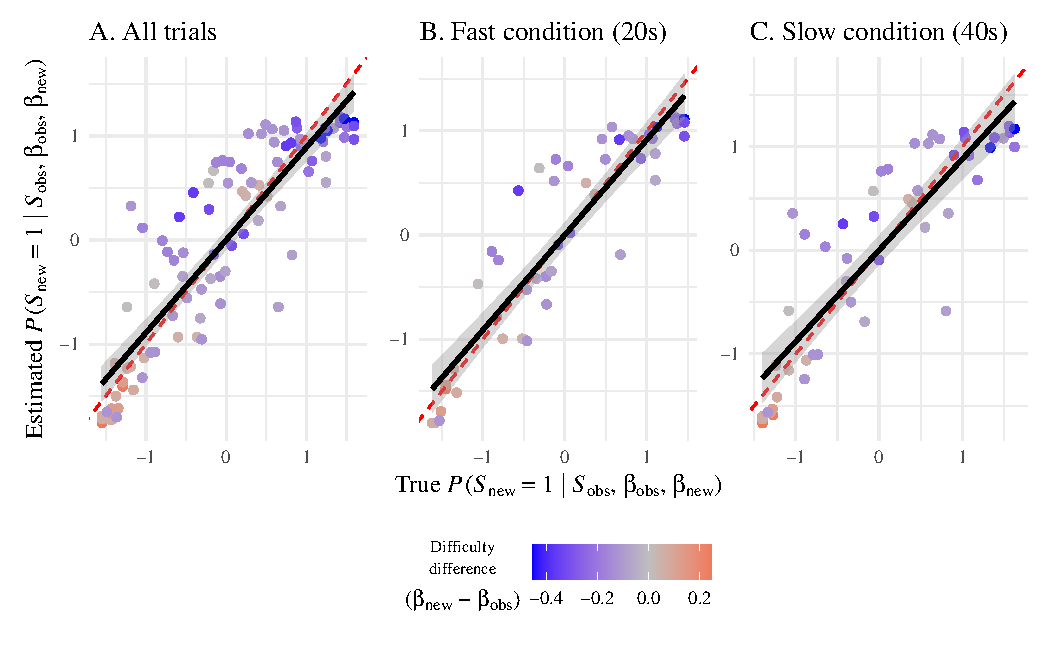
\includegraphics[width=1\linewidth]{../figures/S2-fig-behav-1} 
% 
% }
% 
% \caption{(\textbf{A}) Participants' estimated probability of answering a new question, given performance on a previous question (the observed question), as a function of the true conditional probability, including all trials. (\textbf{B}) Trials in which the observed question is correctly answered. (\textbf{C}) Trials where the observed question is incorrectly answered. Each data point is an observed-new question pair. The red line represents the optimal prediction while the dark line represents the fit of the linear model.}\label{fig:S2-fig-behav}
% \end{figure}

\subsection{Results}
All linear Mixed Models (LMM) were computed with the ``lmerTest'' package to obtain p-values via Satterthwaite's degrees of freedom method (Kuznetsova et al., 2017). For other tests, the R packages used will be specified. For all statistical tests, alpha = 0.05.

All hypotheses and manipulation checks were supported by the participant data and the model comparisons.

Participants, given a single piece of information that another person got a particular arithmetic question right/wrong, were far better than chance at judging which other questions that person would have got right. This inference about the competence of others from very limited information relies on the participants assuming that performance on the arithmetic questions is nested, with people who can answer harder questions also being able to answer easier ones, but not vice-versa. In order to make use of the nestnessness of the questions, participants additionally needed to accurately assess the the rarity of reaching a correct answer in the time limit for different questions, in other words the difficulty of the questions. Our findings suggest that participants were on average able to make all of these judgments, enabling their successful competence inferences.

The arithmetic questions were manipulated to be nested by varying their difficulty. To verify that this manipulation resulted in nestedness of participant performance, two nestedness measures, NODF and Temperature, were calculated from a binary matrix of participants' successes/failures on each question. Each metric was computed using the oecosimu() function in the vegan package in R (Oksanen et al.~2013). The observed nestedness values (NODF or Temperature) were compared to a simulated distribution of possible values under the null hypothesis that the arithmetic questions were not nested. A higher, positive NODF indicates greater nestedness, while a lower, negative Temperature indicates greater nestedness. The primary manipulation check (\textbf{MC1}) was confirmed for both measures, with a significantly higher NODF and lower Temperature than under the null model (NODF: Z = 20.29, p = .002; Temperature: Z = -12.67, p = .002). This confirmed that participants who succeeded on hard questions (rarely answered correctly) also tended to succeed on easier ones (more commonly answered correctly). A secondary manipulation check (\textbf{MC1'}), directly derived from nesting, was then performed to check that, on average, the more difficult the question the higher the average performance score of those who got it right. Fitting a linear model with average performance score as the predictor and objective question difficulty (the rarity of answering correctly within the time limit) as the outcome, the secondary manipulation check was supported as the estimate was significantly positive (\(\beta\) = 0.24, t(13) = 13, p = \textless{} .001, Adjusted \(R^2\) = 0.92).

As a pre-requisite for the participants making use of the nested nature of the questions to infer which questions the virtual agent got right, they must be able to judge the difficulty of the questions. More specifically, they must be able to accurately assess the rarity of reaching an accurate answer within the time-limit for different questions. This was our first hypothesis (\textbf{H1}). We fit a linear mixed effects model predicting true question difficulty (the inverse of the true percentage of people who could answer correctly on the arithmetic test) with participants' perception of the question difficulty (the inverse of the percentage of people they predict could answer correctly) as the fixed effect, and random effects for participants. Confirming \textbf{H1}, the fixed effect estimate for perceived difficulty was significantly positive (\(\beta\) = 0.45, t(911.69) = 22.18, p = \textless{} .001). The high correlation between perceived difficulty and true difficultyis visible in Figure \ref{fig:S1-fig-behav}A.

\begin{figure}

{\centering 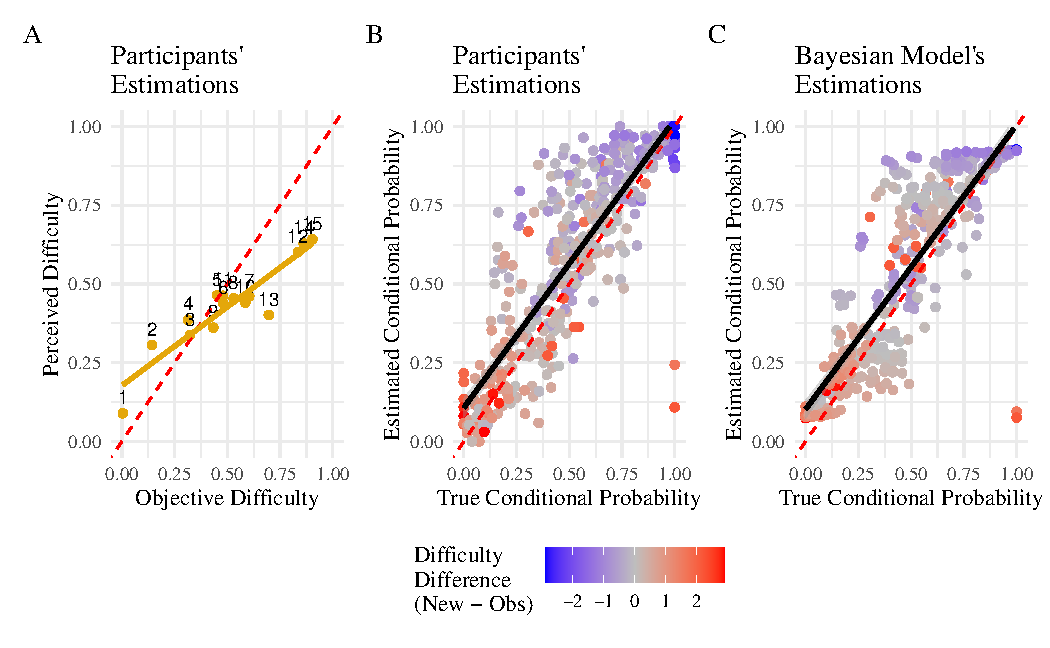
\includegraphics[width=0.9\linewidth]{../figures/S1-fig-behav-1.pdf} 

}

\caption{\textbf{A}: Perceived Difficulty versus Objective Difficulty. Numbers refer to the question ID (see Materials). The red dashed line represents the optimal estimation. \textbf{B}: Estimated Conditional Probability versus True Conditional Probability. Each data point is a pair of two questions. The red line represents the optimal prediction while the dark line represents the fit of the linear model. \textbf{C}: Conditional robabilities estmiated by the Main Model vs True Conditional Probability. Each data point is a pair of two questions. The red line represents the optimal prediction while the dark line represents the fit of the linear model.}\label{fig:S1-fig-behav}
\end{figure}

\section{Study 2}\label{study-2}

Assuming that people are interested in gathering more information about others' competence, are they able to compute the expected amount of information gained if they observe the individual answering a new question, and as a result select the most informative question to ask?

Assessing the rationality of people's information search is typically done by comparing people's choices to a normative model \citep{Dubey-2020, Klayman-1987, Nelson-2005, Oaksford-1994, Tsividis-2014}. We adopt an Optimal Experimental Design (OED) framework \citep{Liefgreen-2020, Nelson-2005, Quillien-2023a}. OED models are composed of two main parts: a specification of the inferences an individual should make given an observation (identified by Study 1), and a measure of the amount of information gained following such an observation.

In this study, we present participants with one piece of information about an individual's competence. We then present participants with a discrete choice task in which they have to choose which new question to ask that individual. The Bayesian model is used to formalize participants' estimation of competence if they asked each question, which allows us to design a normative model to quantify the Expected Information Value of each query. We pre-registered the following hypotheses:

\textbf{H1.} The participants' odds of selecting a query is significantly correlated with the Expected Information Value of the query as computed by the normative model.

\textbf{H2.} Participants' information search behavior depends on the information they have been provided about the previous performance of the individual they are evaluating.

\subsection{Methods}\label{methods-2}

\subsubsection{Participants}\label{participants-2}

We recruited 301 U.S. participants via Prolific; after excluding 5 attention check failures, 296 participants remained (156 women, 140 men, \(M_{age}\) = 39.2, \(SD_{age}\) = 13.4).

\subsubsection{Behavioral task}\label{behavioral-task-2}

Participants were introduced to a virtual individual who had answered, rightly or wrongly, a question on one of three themes. For the observed questions, we used a subset of five questions from the materials of the previous studies. Then, in contrast with the previous studies, participants were told that they had to select an additional question in order to gather more information to assess that individual's level of knowledge or ignorance. Participants were told to imagine that we would give them feedback about whether the individual got the selected question right or wrong. Note that we were interested in which question they would select, so no feedback was provided. They could select one question among a set of six pre-selected questions (one set per theme). We refer to these selectable questions as ``queries.'' This procedure was repeated 10 times: participants were randomly assigned to a theme and were presented to all ten virtual individuals for this theme (each of the five observed questions answered correctly or incorrectly). 
% Figure \ref{fig:fig-overview} provides an illustration of the task.

\subsubsection{Computational Models}\label{computational-models-2}

After observing one performance of the virtual individual, participants had to select which question they would like to reveal in order to improve their estimation of competence. We formalize a normative model with two components: (a) an ideal observer which specifies the inference made after an observation and (b) an ideal search model that scores each candidate query by its Expected Information Value (assuming that inferences is made in the way specified by the ideal observer model).

\textbf{\emph{Ideal observer model.}} The ideal observer model uses the difficulty of the observed question (\(\beta_{obs}\)) and the observed success or failure (\(S_{obs}\)) to update its estimate of competence \(p(\theta \mid \beta_{\text{obs}}, S_{\text{obs}})\). The model is strictly identical to the Bayesian model presented in the previous studies that provide evidence that this model is a good approximation of people's inference. For this study, we do not re-fit the free parameters; instead we use the mean of the best-fitting values from Studies 1 and 2 (the pre-registered values were \(\mu\) = 0.15, \(\sigma^2\) = 0.65 and \(\varepsilon\) = 0.7). Thus, before seeing any information, the model has a prior over competence of \(\theta \sim \mathcal{N}(\mu = 0.15, \sigma^2 = 0.65)\).

\textbf{\emph{Ideal search model.}} The ideal search model aims to quantify the information gained from selecting a query. We assume that once they see a new information (i.e observing a success or failure \(S_{new}\) on a new question of difficulty \(\beta_{new}\)) they will perform a Bayesian update as described in the previous section.

We measure the information gained by observing a new question answered by the virtual individual as the Kullback-Leibler divergence (\(D_{KL}\); Kullback \& Leibler, 1951) of the previous estimation of competence \(p(\theta)\) from the new posterior distribution \(p(\theta')\), given by: \(D_{\text{KL}}(p(\theta') \mid \mid p(\theta)) = \int p (\theta') \text{log}\left( \frac{p(\theta')}{p(\theta)}\right)d\theta'\)

When selecting a query, participants do not yet know how their competence estimation will be affected. However, they can calculate the Expected Information Value (EIV) of each potential query. They do so by simulating two scenarios---one in which the individual answers the new question correctly (\(S_{new}=1\)), and one in which they answer incorrectly (\(S_{new}=0\))---and then weighting these outcomes by their respective probabilities (given their estimation of the difficulty \(\beta_{new}\) of the question). This procedure can be formally expressed as:

\begin{multline}
EIV(Query) = \sum_{s \in \{0,1\}} D_{\text{KL}}\left(p(\theta' \mid \beta_{\text{new}}, S_{\text{new}} = s) \mid \mid p(\theta)\right) \\
\times P(S_{\text{new}} = s \mid \beta_{\text{new}}, \theta)
\label{eq:eiv}
\end{multline}

In summary, the normative model updates its estimation of competence once with the initial observation (\(\beta_{obs}\), \(S_{obs}\)). Then, for each candidate query with difficulty \(\beta_{new}\), it computes the Expected Information Value (Equation \(\ref{eq:eiv}\)) by averaging the information gains over the two possible outcomes (\(S_{new} = \{0,1\}\)).

\textbf{\emph{Alternative ``no-update'' model.}} We also test an alternative ``no-update'' model which is a lesioned version of the normative model. This lesioned variant skips the first step: it ignores the initial observation (\(\beta_{obs}\), \(S_{obs}\)). Instead, it relies on its prior of competence \(p(\theta)\) as its current belief when computing EIV. This prior is the same than the normative model. It still uses the same Ideal Observer likelihood for simulating updates from performance on a new question (\(\beta_{new}\), \(S_{new}\)); it simply does not incorporate the initial observation before selecting a query. Comparing the normative model to this no-update model tests whether people adapt their search given the information presented.

\textbf{\emph{Post-hoc heuristic model.}} In an exploratory analysis, we test a post-hoc model that was not pre-registered. This model predicts that, after observing a correct answer, participants will select harder queries proportionally to their difficulty. Conversely, when observing an incorrect answer, the model predicts the selection of easier questions. Note that this model does not implement a prior over competence, nor does it take into account the difficulty of the observed question. The predicted informational value is the difficulty of the query when observing a correct answer, and minus the difficulty when observing an incorrect answer.

\subsection{Results}\label{results-2}

% \begin{figure}

% {\centering \includegraphics[width=0.8\linewidth]{../figures/fig-model-data-1} 

% }

% \caption{Percentage of choice predicted by the normative model, the no-update model, the heuristic model, and participant's average choice (bottom row), divided by theme and success. The query selections made after the same observation are grouped together by a line and colored in function of the difficulty of the observed question. Each data point corresponds to a pair of a query and an observed question, except for the no-update and heuristic model where the predictions are independent of the observed question. Transformation of the raw difficulty is described in the methods of Study 1. To compare models' predictions with participants choices, we transform $EIV$ values to percentage of choice using a softmax transformation corresponding to bounded-rational (noisy) policy ($\beta$ = 0.5).}\label{fig:fig-model-data}
% \end{figure}

In this discrete choice task, participants had to choose a query among six possible options. Figure \ref{fig:fig-model-data} plots the percentage of choice for each query (conditional on the observed question) compared to the normative model's predictions. Many queries within a given choice set have very similar EIV, so the model's predicted choice probabilities are only weakly differentiated. Under the normative model, EIV is highest for queries whose difficulty is near the estimated competence (i.e., where \(p(S=1) \approx 50\%\), as both a success or a failure would be informative).

To test H1, that participants are more likely to select more informative questions, a mixed multinomial logit model was estimated using the ``mlogit'' package \citep{Croissant-2020} with participant's choice of query as the dependent variable and the EIV for each query (computed with the normative model) as the independent variable. A participant-level random slope on EIV was added to allow the effect of EIV on choice to vary by individual. In accordance with our hypothesis, participants chose high-EIV queries at a rate significantly higher than chance (\(\beta\) = 0.22 \(\pm\) 0.02, \(z\) = 9.42, \(p\) \textless{} .001). In other words, one standard deviation increase in EIV increased the odds of selection by 24\% on average. Participants were quite variable in how optimal they were in choosing the most diagnostic question, with an estimated standard variation in EIV slope between participants of 0.32 \(\pm\) 0.04 (\(z\) = 8.59, \(p\) \textless{} .001). As a descriptive complement to the mixed logit analysis, we computed the rank correlation between query EIV and choice percentage within each trial, then averaged across trials, obtaining a positive but relatively modest correlation (Spearman's \(\rho\) = 0.34).

To test that participants take into account the information previously presented about the individual they are evaluating (H2), we compared our normative model with an alternative ``no-update'' model which does not pay attention to the ``observed question'' (see Figure \ref{fig:fig-model-data}). We fitted a similar mixed multinomial logit model with the EIV predicted by the alternative ``no-update'' model. Participants's choice were not significantly correlated with this alternative estimate for EIV (\(\beta\) = -0.01 \(\pm\) 0.02, \(z\) = -0.67, \(p\) = 0.501). Our normative model explains the data better (\(BIC\) = 10501) than the ``no update'' model (\(BIC\) = 10586).

We tested an alternative heuristic stipulating that when participants observe a correct answer they select harder questions and conversely, they select easier questions when observing an incorrect answer. We fitted another multinomial model with participant's choice as the dependent variable and the predictor was simply the difficulty of the query when observing a correct answer, and minus the difficulty when observing an incorrect answer. We found that participants' choices were significantly predicted by the heuristic (\(\beta\) = 0.23 \(\pm\) 0.02, \(z\) = 10.62, \(p\) \textless{} .001). As before, participants exhibited variation in how their choices followed the heuristic (\(\beta\) = 0.20 \(\pm\) 0.04, \(z\) = 4.78, \(p\) \textless{} .001). This heuristic model provided a marginally better account of the data than the normative model, as indicated by a lower BIC (\(BIC\) = 10495) and a sightly higher mean within-trial rank correlation (Spearman's \(\rho\) = 0.37).

\section{General discussion and conclusion}\label{general-discussion-and-conclusion}

The capacity to infer the competence and knowledge of others is a core component of social cognition. Our main focus was to test whether inferences about competence are consistent with normative Bayesian reasoning but our paradigm also allows us to test whether participants make judgments that approximate objective conditional probabilities well. Study 1 show that people can predict with a high degree of accuracy the conditional probability that a person knows the answer to a trivia question from a minimal amount of information---whether or not they know one other piece of information. This confirms that even a single observation can drive major updates in competence assessment, depending on the diagnosticity of the observed performance (e.g., success on a very difficult item). These studies also provide evidence that inferences of competence are well approximated by a Bayesian model which optimally integrates novel information with prior expectations. By contrast, plausible heuristics, corresponding to lesioned versions of the Bayesian model, do not account as well for most participants' behavior. These two findings---accurate judgments, and reliance on normative inferences---are relatively independent, as applying non-normative heuristics sometimes results in accurate judgments, while normative inferences can produce biased answers when the generative model or the parameters are not well calibrated.

The same Bayesian framework can also explain how people seek information. Study 2 shows that participants are able to flexibly query new information, in a way that can be predicted by an optimal search model based on information theory. The probability of selecting a query was influenced by the normative model Expected Information Value (a measure quantifying the amount of information gained for each candidate query). This result provides convergent evidence across distinct tasks that people's inferences of competence are consistent with a Bayesian model.

On the whole, performance was less in line with the Bayesian model in Study 2 than in Study 1. This difference might stem from the greater computational difficulty of Study 2, in which participants had to compare the potential outcomes of choosing each potential query weighted by the probability of a correct answer. Moreover, the Expected Information Values of each potential query were often similar. In such a situation, it is not surprising that a heuristic approximates participants' behavior (on the rationality of using heuristics for computationally demanding tasks, see \citep{Bramley-2015, Gigerenzer-2011, Wu-2017}).

The present studies have some limitations. The Bayesian model was only tested on inferences of knowledgeability, a specific facet of competence. We believe, however, that the model could be applied to other domains such as estimating technical skills (e.g., using the difficulty of some mental operations to predict numerical competence), or physical feats (e.g., using the effort required to lift an object of a given weight to estimate overall strength). Moreover, the information search task of Study 2 was also particularly difficult; as many questions had similar Expected Information Values, an easier task might have provided a fairer test of the optimal Bayesian model.

Our research opens new directions in understanding the fundamental mechanisms of social cognition. Building on prior literature establishing the importance of past accuracy and difficulty cues, the present research offers a systematic, computational account of how people utilize this information. We show that in a naturalistic paradigm, reliable cues, even if they are minimal, allow participants to form very accurate estimations of competence, in line with Bayesian principles. Future research could address the question of how participants weigh and integrate multiple cues of competence of varying diagnosticity.

\printbibliography

\end{document}
